\section{Global Activity Diagram}

The activity diagram models the dynamic behavior of the system by representing the overall workflow of its core processes \cite{booch2005uml,owler2010uml}. It provides a high-level view of how different actors interact with the system and how operations are executed from start to finish.

\begin{itemize}
	\item The sequence and coordination of activities carried out by each actor
	\item The flow of control between actions, including parallel and synchronized processes
	\item Decision nodes that determine alternative execution paths based on specific conditions
	\item The interaction and data exchange between various system components
\end{itemize}

This diagram provides a global understanding of how the system behaves dynamically and ensures the coherence of the implemented functionalities :

\begin{figure}[H]
	\centering
	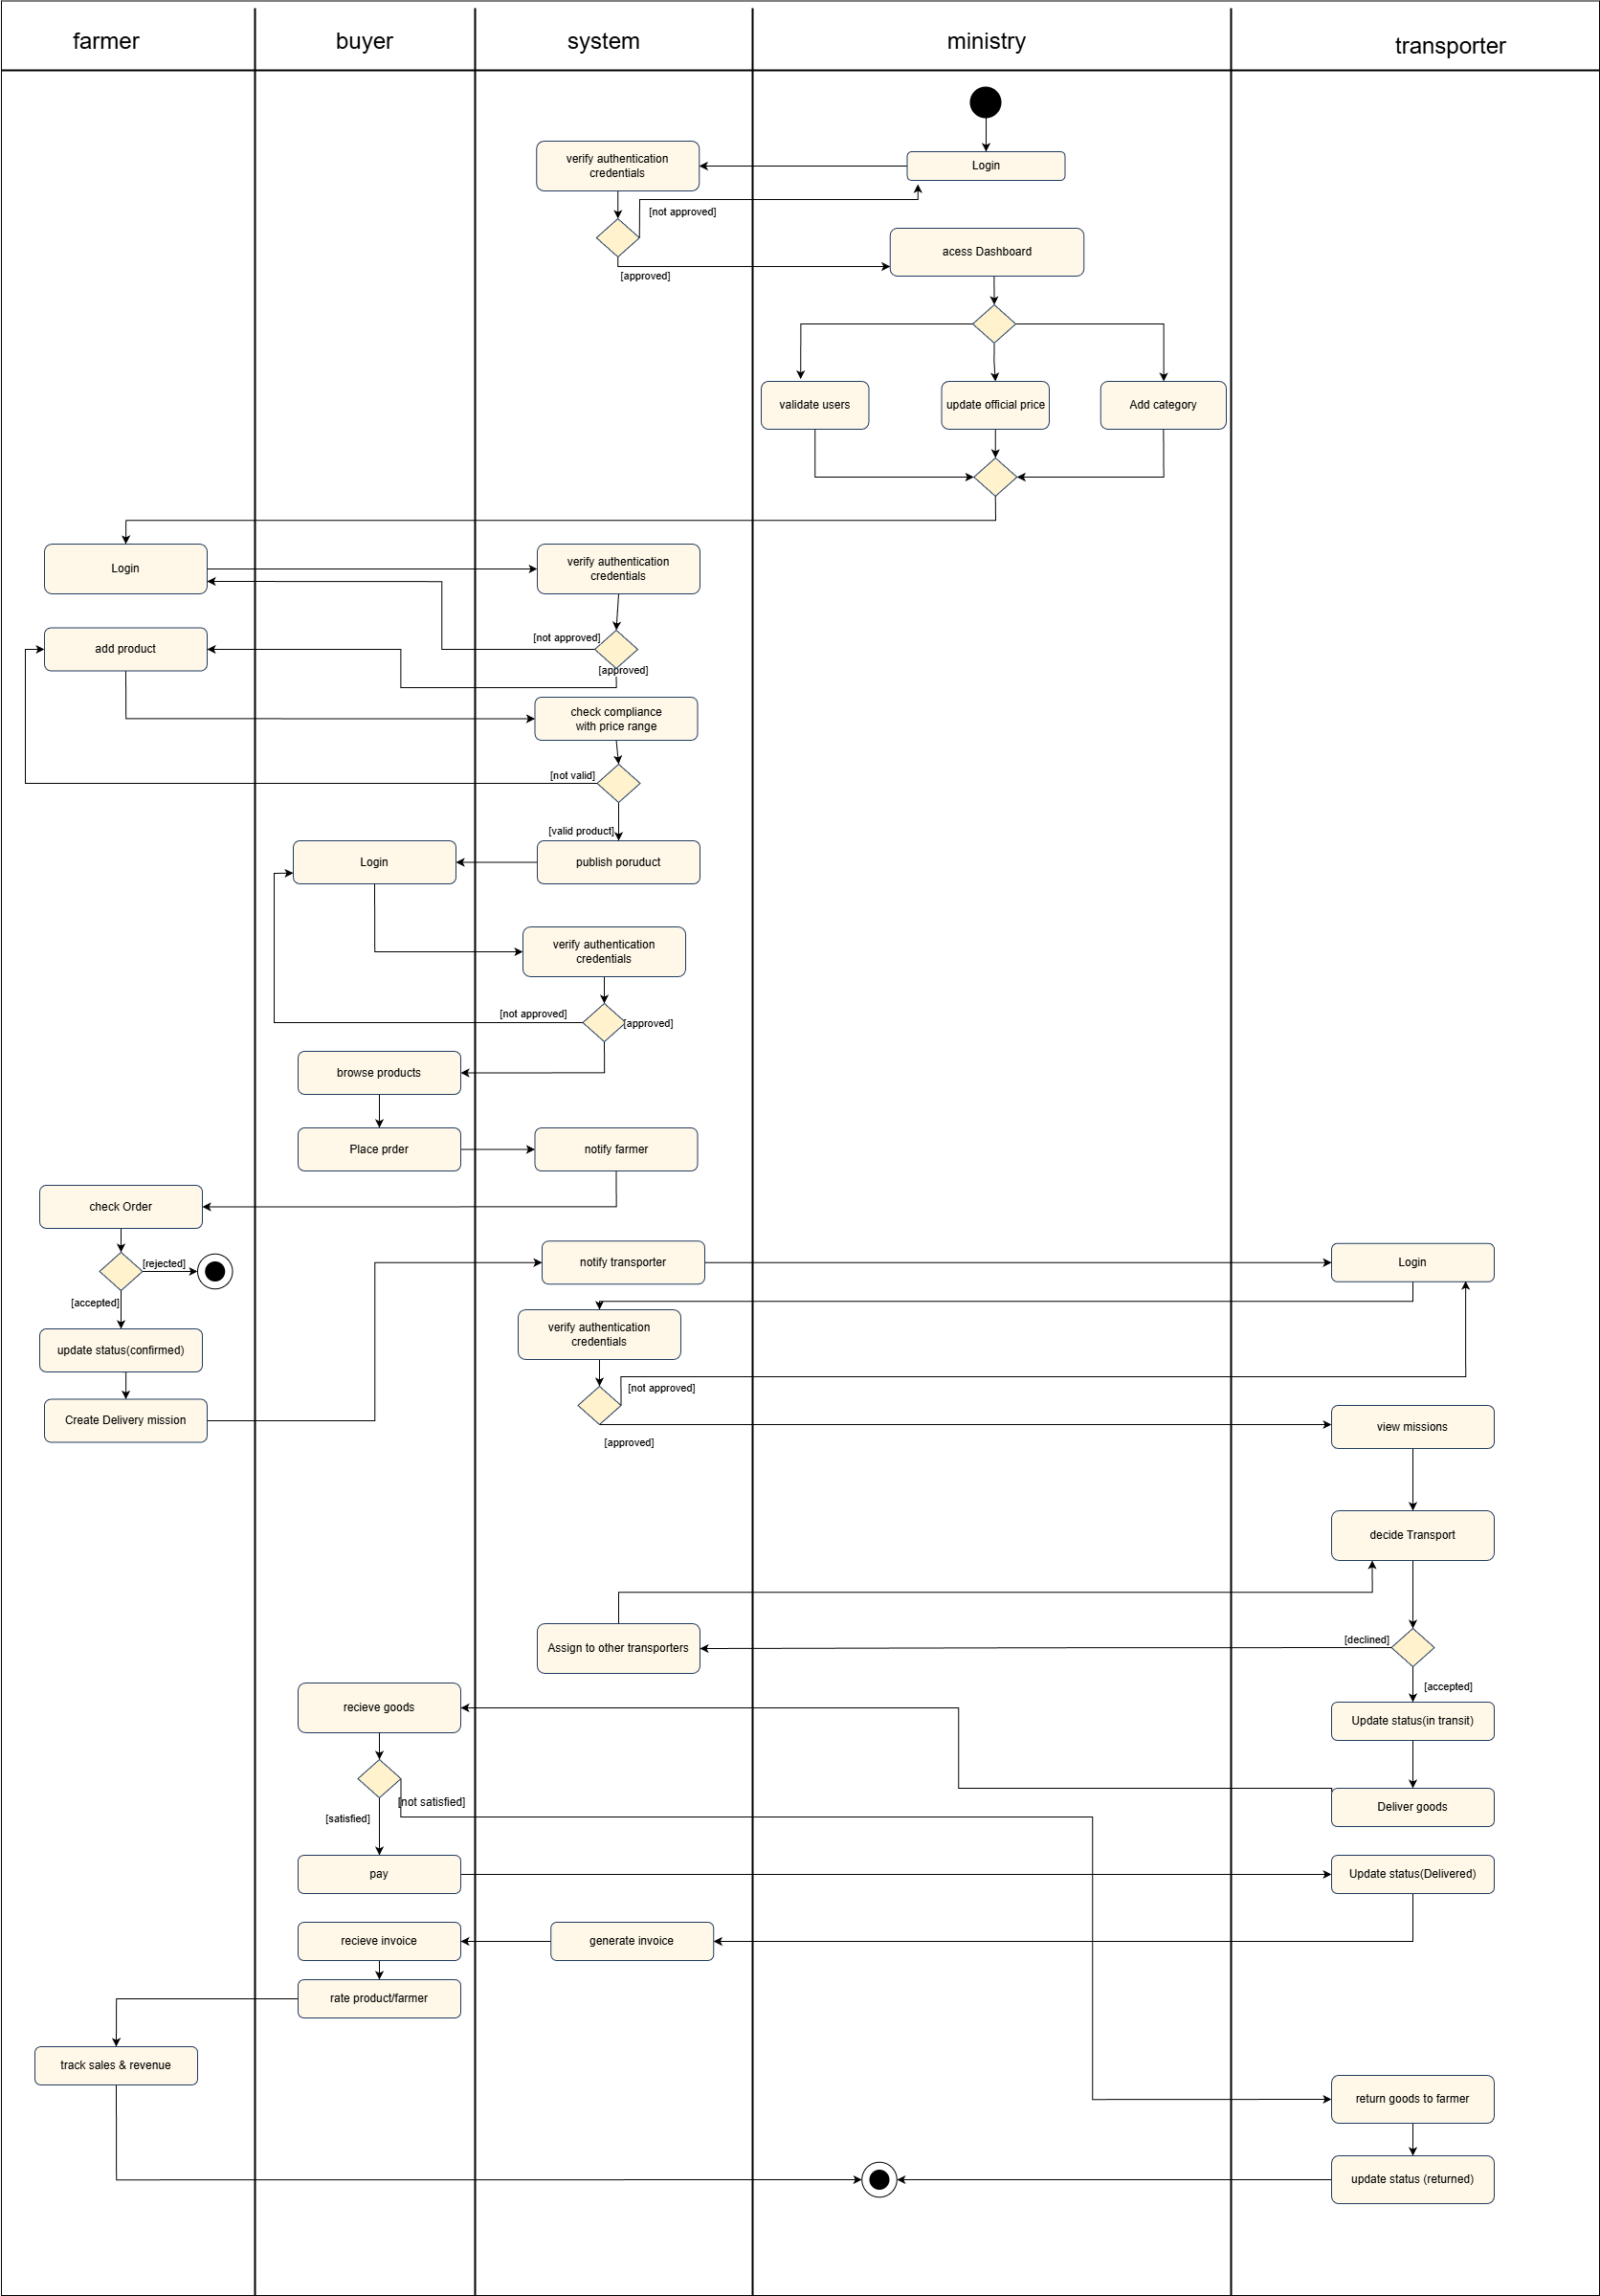
\includegraphics[width=1\linewidth]{images/diagrammes/diagramme_activite}
	\caption{Global Activity Diagram}
\end{figure}

The process begins when a Farmer submits a product listing through the platform. This submission is immediately routed to the Ministry for administrative review. The system the listing to ensure it complies with sector regulations; they have the authority to either reject the listing for corrections or approve it for public display. Once approved by the Ministry, the product becomes visible in the marketplace.

A Buyer then browses the available products and places an order. Following the purchase, the Farmer receives a notification to review and accept the order. Upon acceptance, the system triggers a delivery request to the Transporter network. A Transporter accepts the mission and assigns a specific vehicle to the task.

The Transporter collects the goods from the Farmer and initiates the delivery. The process concludes once the Buyer confirms receipt of the shipment, at which point the farmer can track the previous order and revenue and the buyer can consult his order history.

